\documentclass[12pt]{article}

\usepackage{algorithm}
\usepackage{float}
\usepackage{algpseudocode}
\usepackage{algorithmicx}
\usepackage{algpseudocode}
\usepackage{answers}
\usepackage{authblk}
\usepackage{ctex}
\usepackage{setspace}
\usepackage{graphicx}
\usepackage{enumitem}
\usepackage{multicol}
\usepackage{mathrsfs}
\usepackage[margin=1in]{geometry} 
\usepackage{amsmath,amsfonts,amsthm,amssymb}
\usepackage{mathtools}
\usepackage{multirow}
\usepackage{xcolor}
\usepackage{makecell}
\usepackage{url}
\usepackage{fontspec}
\usepackage{hyperref}
\usepackage[bottom]{footmisc}
\usepackage{hologo}
\usepackage{wallpaper}
\usepackage{makecell}
\usepackage{listings}
\usepackage{xparse}

\NewDocumentCommand{\code}{v}{
	\texttt{\textcolor{blue}{#1}}
}

\lstset{language=bash, keywordstyle={\bfseries \color{blue}}}

\CenterWallPaper{.50}{img/zju_logo.png}
\hypersetup{
    colorlinks=true,
    linkcolor=blue,
	urlcolor=magenta,
	citecolor=red      
}

\newcommand{\ver}{\textmd{Version} 1.0} % Version number.

\newcommand{\mat}[1]{\boldsymbol{#1}}
\newcommand{\spc}[1]{\textit{#1}}
\renewcommand{\vec}[1]{\boldsymbol{#1}}

\newcommand{\N}{\mathbb{Z}^+}
\newcommand{\Z}{\mathbb{Z}}
\newcommand{\Q}{\mathbb{Q}}
\newcommand{\Qp}{\mathbb{Q}^+}
\renewcommand{\C}{\mathbb{C}}
\newcommand{\R}{\mathbb{R}}
\newcommand{\F}{\textit{F}}
\newcommand{\T}{\textit{T}}
\renewcommand{\P}{\textit{P}}
\newcommand{\J}[1]{\textit{J}_{\mat{#1}}}
\newcommand{\V}{\spc{V}}
\newcommand{\E}{\spc{E}}
\renewcommand{\L}{\mathcal{L}}

\newcommand{\inv}{^{\mathsf{-1}}}
\newcommand{\herm}{^{\mathsf{H}}}

\newcommand{\adj}[1]{\operatorname{adj}(\mat{#1})}
\DeclareMathOperator{\spn}{span}
\DeclareMathOperator{\rnk}{rank}
\DeclareMathOperator{\nul}{nullity}
\DeclareMathOperator{\Ker}{N} % Capital, since \ker is already defined.
\DeclareMathOperator{\lker}{Lker}
\DeclareMathOperator{\im}{Im}
\DeclareMathOperator{\cs}{CS}
\DeclareMathOperator{\rs}{RS}
\DeclareMathOperator{\tr}{tr}
\DeclareMathOperator{\cof}{cof}
\DeclareMathOperator{\am}{am}
\DeclareMathOperator{\gm}{gm}
\DeclareMathOperator{\len}{Length}
\DeclareMathOperator{\num}{Number}
\newcommand{\ii}{{i\mkern1mu}}
\newcommand{\dotp}[2]{<#1, #2>}
\newcommand{\proj}[2]{\operatorname{proj}_{#1}\vec{#2}}
\newcommand{\Mod}[1]{\ (\mathrm{mod}\ #1)}
\DeclarePairedDelimiter{\ceil}{\lceil}{\rceil}
\DeclarePairedDelimiter{\floor}{\lfloor}{\rfloor}

\newcommand{\tnr}{\fontspec{Times New Roman}}
\newcommand{\con}{\fontspec{Consolas}}
 
\newenvironment{theorem}[2][Theorem]{\begin{trivlist}
\item[\hskip \labelsep {\bfseries #1}\hskip \labelsep {\bfseries #2}]}{\end{trivlist}}

\renewcommand{\contentsname}{Table of Contents}
\renewcommand{\refname}{References}
\renewcommand{\tablename}{Table}
\renewcommand{\figurename}{Figure}

\begin{document}

\title{\Huge{\textbf{作業系統}} \\
	\LARGE{\textbf{Operating System}}
}
\newcommand*{\affaddr}[1]{#1}
\newcommand*{\affmark}[1][*]{\textsuperscript{#1}}
\author{
	TZU-CHUN HSU\affmark[1] \\
	\affmark[1]\href{mailto:vm3y3rmp40719@gmail.com}{vm3y3rmp40719@gmail.com} \\
	\affaddr{\affmark[1]Department of Computer Science, Zhejiang University
	}
}

\date{\mbox{}\vfill\today\\ \ver}

\maketitle
\pagebreak

\addcontentsline{toc}{section}{Disclaimer}
\begin{center}
    \Huge{\texttt{Disclaimer}}\\
\end{center}

本文「演算法」為台灣研究所考試入學的「演算法」考科使用,內容主要參考洪捷先生的演算法參考書\cite{1},以及wjungle網友在PTT論壇上提供的演算法筆記\cite{2}。 \\
本文作者為\textsc{TZU-CHUN HSU},本文及其\hologo{LaTeX}相關程式碼採用\textbf{MIT協議},更多內容請訪問作者之\textsc{GitHub}分頁\href{https://github.com/Oscarshu0719}{Oscarshu0719}。 \\~\\

\con
MIT License

Copyright (c) 2020 TZU-CHUN HSU

Permission is hereby granted, free of charge, to any person obtaining a copy
of this software and associated documentation files (the "Software"), to deal
in the Software without restriction, including without limitation the rights
to use, copy, modify, merge, publish, distribute, sublicense, and/or sell
copies of the Software, and to permit persons to whom the Software is
furnished to do so, subject to the following conditions:

The above copyright notice and this permission notice shall be included in all
copies or substantial portions of the Software.

THE SOFTWARE IS PROVIDED "AS IS", WITHOUT WARRANTY OF ANY KIND, EXPRESS OR
IMPLIED, INCLUDING BUT NOT LIMITED TO THE WARRANTIES OF MERCHANTABILITY,
FITNESS FOR A PARTICULAR PURPOSE AND NONINFRINGEMENT. IN NO EVENT SHALL THE
AUTHORS OR COPYRIGHT HOLDERS BE LIABLE FOR ANY CLAIM, DAMAGES OR OTHER
LIABILITY, WHETHER IN AN ACTION OF CONTRACT, TORT OR OTHERWISE, ARISING FROM,
OUT OF OR IN CONNECTION WITH THE SOFTWARE OR THE USE OR OTHER DEALINGS IN THE
SOFTWARE.

\tnr
\pagebreak

\section{Overview}

\begin{enumerate}
    \item 本文頁碼標記依照實體書\cite{1}\cite{2}的頁碼。
    \item TKB筆記\cite{3}章節頁碼:
    \begin{table}[H]
        \centering
        \begin{tabular}{|c|c|}
            \hline
            Chapter & Page No. \\
            \Xhline{2\arrayrulewidth}
            1 & 1 \\
            \hline
            2 & 27 \\
            \hline
            3 & 81 \\
            \hline
            4 & 101 \\
            \hline
            5 & 119 \\
            \hline
            6 & 165 \\
            \hline
            7 & 221 \\
            \hline
            8 & 238 \\
            \hline
        \end{tabular}
    \end{table}
    \item 常考:(參考TKB筆記\cite{3}中頁碼)
    \begin{enumerate}
        \item 19 
        \item 59
        \item 84
        \item 92
        \item 141
        \item 170
        \item 200
    \end{enumerate}
    \item 省略第一章重點十四,第二章重點五、六、十,第六章重點十四,第七章只看重點一到四及十,第八章重點五一致性協定範例。
\end{enumerate}

\pagebreak
\begingroup
\section{Summary}
\begin{enumerate}
\let\clearpage\relax
\item \begin{theorem}{(1.6)} $\phi$為任何集合的子集。
\end{theorem}

\item \begin{theorem}{(1.16)} \begin{subequations}
    \begin{align}
        \P(A \cup B) & \neq \P(A) \cup \P(B) \\
        \P(A \cap B) & = \P(A) \cap \P(B)
    \end{align}
    \end{subequations}
\end{theorem}

\item \begin{theorem}{(1.55)} 若$a, b, c \in \N$,則$ax + by = c$有整數解$\iff$$\gcd(a, b) | c$。
\end{theorem}

\item \begin{theorem}{(1-42)1.92} $2^{mn} \Mod{2^m - 1} = 1$。
\end{theorem}

\item \begin{theorem}{(1.58, 1.60)} (質數)
    \begin{itemize}
        \item 若$a \in \Z, n \in \N$,且$\gcd(a, n) = 1$,則$a^{-1} \Mod{n}$存在。
        \item 若$p$為質數,$a \in \Z$,則$a^{-1} \equiv a \Mod{p}$即$a^2 \equiv 1 \Mod{p}$$\iff$$a \equiv \pm 1 \Mod{p}$。
    \end{itemize}
\end{theorem}

\item \begin{theorem}{(1.62)} 若$a, b, c, n \in \Z$,若$\gcd(c, n) = 1$,則$ac \equiv bc \Mod{n}$$\iff$$a \equiv b \Mod{n}$。
\end{theorem}

\item \begin{theorem}{(1.61, 1.62)} (質數)
    \begin{itemize}
        \item Wilson's theorem:
        若$p$為質數,則
        \begin{equation}
            (p - 1)! \equiv -1 \Mod{p}
        \end{equation}
        \item Fermat's little theorem:
        若$p$為質數,$m \in Z$,且$\gcd(m, p) = 1$,則
        \begin{equation}
            m^{p - 1} \equiv 1 \Mod{p}
        \end{equation}
    \end{itemize}
\end{theorem}

\item \begin{theorem}{(1.64, 1.65, 1.66)} (質數)
    \begin{itemize}
        \item 若$n \in \N$,則Euler $\phi$-函數$\phi(n)$為$\{1, 2, \ \cdots, n - 1\}$中與$n$互質的元素個數,又稱Euler's totient function。
        \item 若$n = p_1^{e_1}p_2^{e_2}\cdots p_k^{e_k}$為$n$的質因數分解,則$\phi(n) = n\PI_{j = 1}^{k}(1 - \frac{1}{p_j})$。
        \item 若$p \in \N$,則$\phi(p) = p - 1$$\iff$$p$為質數。
        \item 若$m \in \Z, n \in \N$,且$\gcd(m, n) = 1$,則$m^{\phi(n)} \equiv 1 \Mod{n}$。
        \item 若$p$為質數,$m \in Z$,且$\gcd(m, p) = 1$,則$m^{-1} \equiv m^{p - 2} \Mod{p}$
    \end{itemize}
\end{theorem}

\item \begin{theorem}{(1.66)} 中國餘數定理(Chinese Remainder Theorem,CRT)中,模的數之間必須互質。
\end{theorem}

\item \begin{theorem}{(1.71)} RSA公鑰密碼系統(RSA public key cryptosystem):\begin{itemize}
        \item 訊息:$M$。
        \item 加密鑰(encryption key):\begin{equation}
            n = pq, \ e
        \end{equation}
        其中$p, q$為質數,且$\gcd(e, \phi(n)) = 1, \ \phi(n) = (p - 1)(q - 1)$。
        \item 加密訊息:\begin{equation}
            C = M^e \Mod{n}
        \end{equation}
        \item 解密鑰(decryption key):\begin{equation}
            d \equiv e^{-1} \Mod{\phi(n)}
        \end{equation}
        \item 解密訊息:\begin{equation}
            C^d \equiv M \Mod{n}
        \end{equation}
    \end{itemize}
\end{theorem}

\item \begin{theorem}{(2.51)} (可逆)若$\mat{A}$為可逆上三角矩陣,則$\adj{A}$和$\mat{A}\inv$也是上三角矩陣。
\end{theorem}

\item \begin{theorem}{((2-45)2.92)} (可逆,方陣)若$\mat{A}, \mat{B} \in \F^{n \times n}$為可逆方陣,則$\adj{\mat{AB}} = \adj{\mat{B}}\adj{\mat{A}}$。
\end{theorem}


\begin{theorem}{(60, 61)} Process life cycles (Figure \ref{img:process_lifecycles}): \begin{itemize}
        \item State:\begin{itemize}
            \item New (Created):Process is created and PCB is allocated in kernel, but memory space is NOT allocated.
            \item Ready:Process is allocated memory space.
        \end{itemize}
        \item Transition:\begin{itemize}
            \item Admitted:Process is allocated memory space. In batch system, use long-term scheduler to decide which process to load into memory. In time-sharing and real-time systems, do NOT use long-term scheduler.
            \item Dispatch:Short-term (CPU) scheduler decides which process to get CPU allocation and allocates CPU to execute.
            \item Interrupt (Time-out):e.g. time-out interrupt.
        \end{itemize}
        \item Zombie state:Process is finished, but the parent process have NOT collected results of the children processes, or parent process have NOT executed wait() system call. Resources are released, but PCB have NOT been deleted, until parent process collects the results, then kernel delete PCB.
    \end{itemize}
\end{theorem}

\begin{figure}[H]
    \centering
    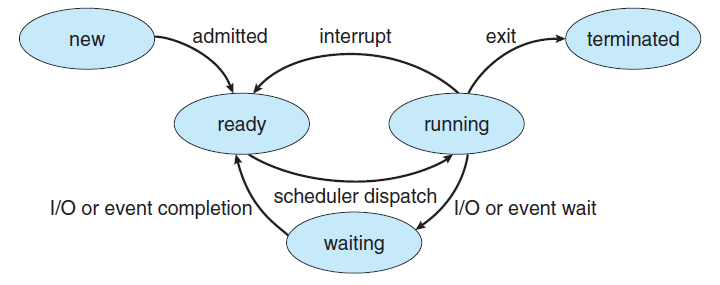
\includegraphics[scale=0.8]{img/process_lifecycles.png}
    \caption{Process life cycles.}
    \label{img:process_lifecycles}
\end{figure}

\begin{theorem}{(67)} Scheduler:\begin{itemize}
        \item Long-term (Job) scheduler:通常batch system採用,time-sharing與real-time systems不採用,從job queue中選jobs載入memory。執行頻率最低,可以調控multiprogramming degree與CPU-bound與I/O-bound jobs的比例。
        \item Short-term (CPU, process) scheduler:從ready queue選擇一個process分派給CPU執行。所有系統都需要,執行頻率最高,\textbf{無法}調控multiprogramming degree與CPU-bound與I/O-bound jobs的比例。
        \item Medium-term scheduler:Memory space不足且有其他processes需要更多memory時執行,選擇Blocked或lower priority process swap out to disk。Time-sharing system採用,batch和real-time systems不採用,可以調控multiprogramming degree與CPU-bound與I/O-bound jobs的比例。
    \end{itemize}
\end{theorem}

\begin{theorem}{(69, 70)} \quad\quad \begin{itemize}
        \item Context switch:\begin{itemize}
            \item 執行期間無法執行process,主要取決於硬體因素。
            \item 降低負擔:\begin{itemize}
                \item 提供Multiple registers set:每個process有自己的registers set,只需要切換pointer就能context switch。
                \item 使用Multi-threading。
            \end{itemize}
        \end{itemize}
        \item Dispatcher:\begin{itemize}
            \item 將CPU真正分配給CPU scheduler選擇的process。
            \item Context switch.
            \item Switch mode to user mode.
            \item Jump to execution entry of process.
        \end{itemize}
    \end{itemize}
\end{theorem}

\begin{theorem}{(63)} Process control operation: \begin{itemize}
        \item \code{fork()}:\begin{itemize}
            \item child process有與parent process不同的memory space,而起始code section和data section皆來自parent process的複製。
            \item 失敗:回傳負值;成功:回傳$0$給child process,$> 0$值即child process PID給parent process。
        \end{itemize}
        \item \code{wait()}:若child process已終止,帶parent process還沒執行$wait()$,但kernel含不能清除child process PCB,直到parent process收集完child process info,此段期間稱zombie。
        \item \code{execlp(dir, filename, args)}:載入特定工作執行,memory content不再是parent process的複製,沒有參數填\code{NULL},e.g. \code{execlp("/bin/ls", "ls", NULL)}。
    \end{itemize}
\end{theorem}

\begin{theorem}{(70)} 評估scheduling performance: \begin{itemize}
        \item Waiting time:Process在\textbf{ready queue}的時間。
        \item Turnaround:Process\textbf{進入系統到完成工作}的時間。
        \item Response time:User輸入到系統產生第一個回應的時間。
    \end{itemize}
\end{theorem}

\begin{theorem}{(75)} Starvation:\begin{itemize}
        \item 有機會完成但是機會很小。
        \item 通過Aging解決:當process在系統中時間增加,逐漸提升process的prioirty。但是soft real-time systems不能使用Aging,因為會違反定義。
    \end{itemize}
\end{theorem}

\begin{theorem}{(71, 72, 75, 76, 77, 78)} Scheduling algorithms: \begin{itemize}
        \item FCFS (First-come-first-serve):可能遭遇Convoy effect,即許多processes都在等待一個需要很長CPU time的process完成工作。
        \item SJF (Shortest-Job-First):\begin{itemize}
            \item Preemptive SJF又稱SRTF (Shortest-Remaining Time First)。
            \item 效益最佳(包含SRTF),即平均等待時間最短。
            \item 對long-burst time job,可能有starvation。
            \item 不適合用在CPU (short-term) scheduling,因為不知道process的精確next CPU burst time,短時間也難以精準預估。
            \item Long-term job可能可行。
            \item Exponential Average:預估next CPU burst time。\begin{equation}
                \tau_{n + 1} = \alpha t_n + (1 - \alpha)\tau_n
            \end{equation} 其中,$t_n$為本次CPU實際值,$\alpha$為機率。
        \end{itemize}
        \item Round-Robin (RR) scheduling:\begin{itemize}
            \item Time-sharing system採用。
            \item 效能取決於time quantum大小,太小context switch太頻繁。
            \item Time quantum大小會影響turnaround time,平均turnaround time\textbf{未必}會隨著quantum time增加而下降。
        \end{itemize}
        \item Multi-level queue (MQ):\begin{itemize}
            \item Queue之間採用fixed priority preemptive scheduling或RR。
            \item 每個queue有各自的scheduling。
            \item \textbf{不}允許process在queues間移動,因此缺乏彈性。
            \item 易starvation,且無法通過類似Aging改善。
        \end{itemize}
        \item Multi-level feedback queue (MFQ):\begin{itemize}
            \item 允許process在queues間移動,可降級增加彈性。
            \item No starvation,可以採用Aging防止starvation。
        \end{itemize}
        \item Priority scheduling:\begin{equation}
            \begin{aligned}
                \text{FCFS}, \text{SJF}, \text{SRTF} & \subset \text{Priority} \\
                \text{FCFS} & \subset \text{RR} \\
                \text{FCFS}, \text{SJF}, \text{SRTF}, \text{Priority}, \text{RR}, \text{MQ} & \subset \text{MFQ}
            \end{aligned}
        \end{equation}
        \begin{table}[H]
            \centering
            \begin{tabular}{|c|c|c|c|c|}
                \hline
                Scheduling & 公平 & Preemptive & Non-preemptive & Starvation \\
                \Xhline{2\arrayrulewidth}
                FCFS & $\surd$ & & $\surd$ & \\
                \hline
                SJF & & & $\surd$ & $\surd$ \\
                \hline
                SRTF & & $\surd$ & & $\surd$ \\
                \hline
                Priority & & $\surd$ & $\surd$ & $\surd$\\
                \hline
                RR & $\surd$ & $\surd$ & & \\
                \hline
                MQ & & $\surd$ & & $\surd$ \\
                \hline
                MFQ & & $\surd$ & & \\
                \hline
            \end{tabular}
        \end{table}
    \end{itemize}
\end{theorem}

\begin{theorem}{(79)} Multiprocessors system:\begin{itemize}
        \item \begin{itemize}
            \item ASMP:類似single-CPU scheduling。
            \item SMP:\begin{itemize}
                \item 所有CPU共用一條ready queue,no load balancing problem,須防止race condition。
                \item 每一個CPU有各自ready queue,可能有load balancing problem,可以通過kernel協調imbalance CPUs給其他ideal CPUs processes。
            \end{itemize}
        \end{itemize}
        \item Processor affinity:\begin{itemize}
            \item 一但process在某CPU上執行,盡量避免migration。
            \item 因為migration from one CPU to another,first CPU cache should be invalidated and second CPU cache should be repopulated, and it costs a lot。
            \item Migrating a process may incur a penalty on NUMA systems, where a process may be moved to a CPU that requires longer memory access time。
        \end{itemize}
        \item Multicores:有Memory stall problem。\begin{itemize}
            \item 通過Multithreaoded processing cores解決,2 or more hardware threads are assigned to each core。
            \item 當一thread memory stall,core can switch to another thread。
            \item 每個thread OS視為logical CPU,皆可執行software thread (process),稱為Cheap Multithreading Technology (CMT)。
        \end{itemize}
    \end{itemize}
\end{theorem}

\begin{theorem}{(80)} Real-time system:\begin{itemize}
        \item Soft real-time system:\begin{itemize}
            \item 採用preemptive和priority scheduling,不提供aging。
            \item Minimize latency:包含interrupt latency和dispatch latency (Figure \ref{img:real_time_dispatch}),real-time system不適合non-preemptive;若是preemptive,須防止race condition。
            \item Prioity inversion:Higher priority process waits for lower priority process to release resources. 通過Priority inheritance解決:讓lower priority process暫時繼承higher priority,以便盡快取得CPU執行,完成後再恢復lower priority。
            \begin{figure}[H]
                \centering
                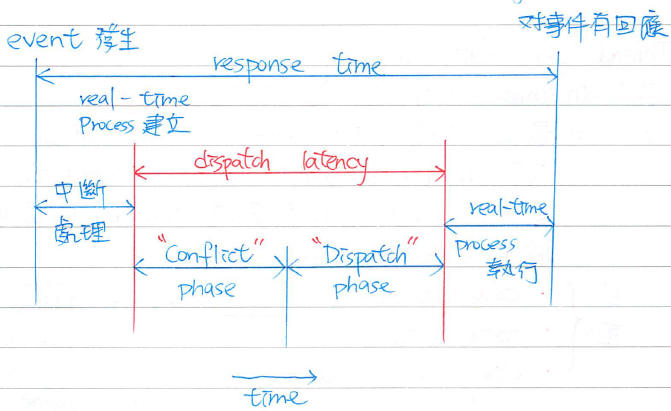
\includegraphics[scale=0.8]{img/real_time_dispatch.png}
                \caption{Dispatch latency on real-time systems.}
                \label{img:real_time_dispatch}
            \end{figure}
        \end{itemize}
    \end{itemize}
\end{theorem}

\begin{theorem}{(80)} Hard real-time system:\begin{itemize}
        \item 討論Synchronous real-time event scheduling,即每隔一段時間發生,需在deadline前完成。
        \item Schedulable判斷:\begin{equation}
            \sum_{i = 1}^{n} \frac{c_i}{p_i} \le 1
        \end{equation} 若符合則schedulable。其中,$n$為事件數目,$c_i$為CPU burst time,$p_i$為period time。
        \item Process meets deadline scheduling algorithms:\begin{itemize}
            \item Rate-Monotonic:\begin{itemize}
                \item Static priority且preemptive。
                \item Period time越小,則priority越高。
                \item Under schedulable,也\textbf{不能}保證所有event皆滿足deadline。
                \item 若其無法滿足deadline,其他static priority scheduling也無法。
            \end{itemize}
            \item EDF (Earliest Deadline First):\begin{itemize}
                \item Dynamic priority且preemptive。
                \item Deadline越小,則priority越高。
                \item Under schedulable,保證所有event皆滿足deadline。
                \item CPU utilization不可能達到$100\%$。
            \end{itemize}
        \end{itemize}
    \end{itemize}
\end{theorem}

\begin{theorem}{(86)} Thread:\begin{itemize}
        \item 又稱Lightweight process。
        \item process是OS分配\textbf{resources}的基本單位,而thread是OS分配\textbf{CPU time}的基本單位。
        \item 同一process之threads共享process的data section (static local and global variables)、heap和code section等,在同一個address可以有多個threads同時執行。
        \item 若一thread被blocked,則CPU可切換給其他thread執行,所以process不會blocked。
        \item Private contents較traditional prcocess少,context switch較快。
        \item 同一process的不同threads可以平行在不同CPUs上執行。
        \item 種類:\begin{itemize}
            \item User-level thread:\begin{itemize}
                \item 由在user site的thread library管理,不需要kernel管理,e.g. POSIX的pthread library,但只是提供規格並沒有實現。
                \item Kernel不知道其存在,因此kernel不干預,導致不同threads\textbf{無法}平行在不同CPUs上執行。
                \item 若user thread發出blocking system call時,則該process也會被blocked,即時該process還有其他available threads。
            \end{itemize}
            \item Kernel-level thread:現行OS皆支持。
        \end{itemize}
        \item pthread library is provided by user-level or kernel-level.
        \item Windows Thread library and Java Thread library are kernel-level threads.
    \end{itemize}
\end{theorem}

\begin{theorem}{(88)} Thread model (user thread-to-kernel thread):\begin{itemize}
        \item Many-to-One model:即user-level thread。
        \item One-to-One model:\begin{itemize}
            \item Not efficient than Many-to-One model.
            \item 若建立過多user thread,kernel overhead過重,performance下降,一般會限制thread數量。
            \item e.g. Linux, family of Windows OS, OSX.
        \end{itemize}
        \item Many-to-Many model:\begin{itemize}
            \item Overhead較One-to-One小,但製作較複雜。
            \item NOT efficient than Many-to-One model.
            \item e.g. Solaris 2,但它是用two-level mapping model製作,同時也允許One-to-One。
        \end{itemize}
    \end{itemize}
\end{theorem}

\begin{theorem}{(90)} Threading issues:\begin{itemize}
        \item \code{fork()} issue:若parent和child thread工作相同,則複製parent process所有threads到child thread;反之,則只複製該thread到child process。
        \item Signal delivery issue: \begin{itemize}
            \item 種類:\begin{itemize}
                \item Synchronous:自作自受,e.g. Divide-by-zero。
                \item Asynchronous:池魚之殃,e.g. aborted by system admin, parent被終止,child也一同被終止。
            \end{itemize}
            \item Signal delivery:\begin{itemize}
                \item Deliver signal to the thread to which the signal applies, e.g. synchronous signal.
                \item Deliver signals to all threads, e.g. user abortion.
                \item Deliver signals to some threads, e.g. kill.
                \item Assign a specific thread to receive all signals for its process, e.g. Solaris 2. 
            \end{itemize}
        \end{itemize}
    \end{itemize}
\end{theorem}

\end{enumerate}
\endgroup
\bibliographystyle{plain}
\bibliography{content/bibliography}
\addcontentsline{toc}{section}{References}


\end{document}
